\makeatletter\let\ifGm@compatii\relax\makeatother
\documentclass[red]{beamer}

%\usepackage{beamerthemesplit}
\usepackage{listings}
\usepackage{comment}
\usepackage{url}
\usepackage{bm}
\usepackage{amsmath}
\usepackage{tikz}
\usetikzlibrary{arrows.meta}
\usetikzlibrary{shapes.symbols}

\usepackage{hyperref} % has to be last
\hypersetup{
    colorlinks=true,
    linkcolor=blue,
    filecolor=magenta,      
    urlcolor=cyan,
    pdfpagemode=FullScreen,
    }

\tikzset{
    saiarrow/.style={{-Latex}, thick}
}

\newcommand{\isred}[1]{{\color{red} {\bf #1}}} 
\newcommand{\isblue}[1]{{\color{blue}{\bf #1}}} 
\newcommand{\isgreen}[1]{{\color{green} {#1}}} 
\newcommand{\isdarkgreen}[1]{{\color{darkgreen} {#1}}} 
\newcommand{\isorange}[1]{{\color{orange} {#1}}} 

\newcommand{\N}{\mathbb N}
\newcommand{\Z}{\mathbb Z}
\newcommand{\Q}{\mathbb Q}
\newcommand{\R}{\mathbb R}

\begin{document}


\setbeamercolor{alerted_text}{fg=cyan}
\xdefinecolor{purplish}{cmyk}{0.75,0.75, 0, 0}
\xdefinecolor{purple}{cmyk}{0.75,0.75, 0, 0}
\colorlet{newred}{red!60!black}

\title{Session 5: Diffie-Hellman}
\author{Slides prepared by UMBC Protocol Analysis Lab}
\date{Last edited \today}
\begin{frame}
\maketitle
\end{frame}

\begin{frame}\frametitle{How do we actually use encryption?}
\begin{figure}
    \centering
    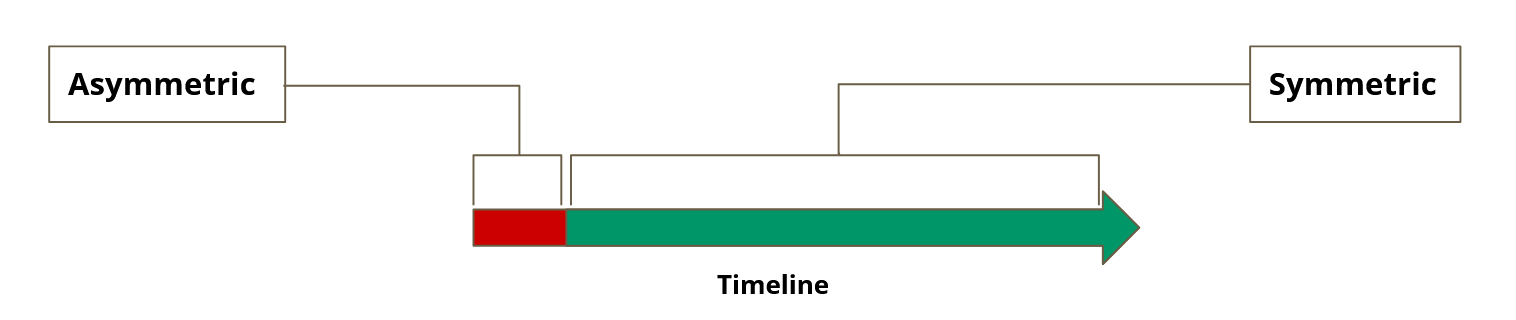
\includegraphics[width=1\linewidth]{slide-images/hybrid-kex.png}
\end{figure}
\end{frame}

\begin{frame}\frametitle{Generators}
\pause
Let \(p\) be a prime, and \(g \in \{1, \dots, p-1\}\).

\pause
\begin{definition}
\(g\) is a \emph{generator} for\(\mod p\) if:
\[
(\{g^1,\dots,g^{(p-1)}\} \mod p) = \{1,\dots,p-1\}
\]
This set $\{ 1, \dots , p-1\}$ on multiplication is known as \(\Z_p^\times\)
\end{definition}
\pause
We can represent a generator in CPSA as \texttt{(gen)}, \\
or \texttt{(exp (gen) (one))}.

\pause
Note that \texttt{(gen)} is a term itself in CPSA.
\end{frame}

\begin{frame}\frametitle{Exponents}
    \pause
    Recall the exponent property
    \[
    x^a \times x^b = x^{a\times b}
    \]
    \pause
    Diffie-Hellman takes advantage of this property by letting us intelligently choose \(a\) and \(b\).
    \pause
    We call these exponent terms \(a\) and \(b\) random exponents, with \emph{sort} \texttt{rndx}.

\end{frame}

\begin{frame}
\begin{figure}
    \centering
    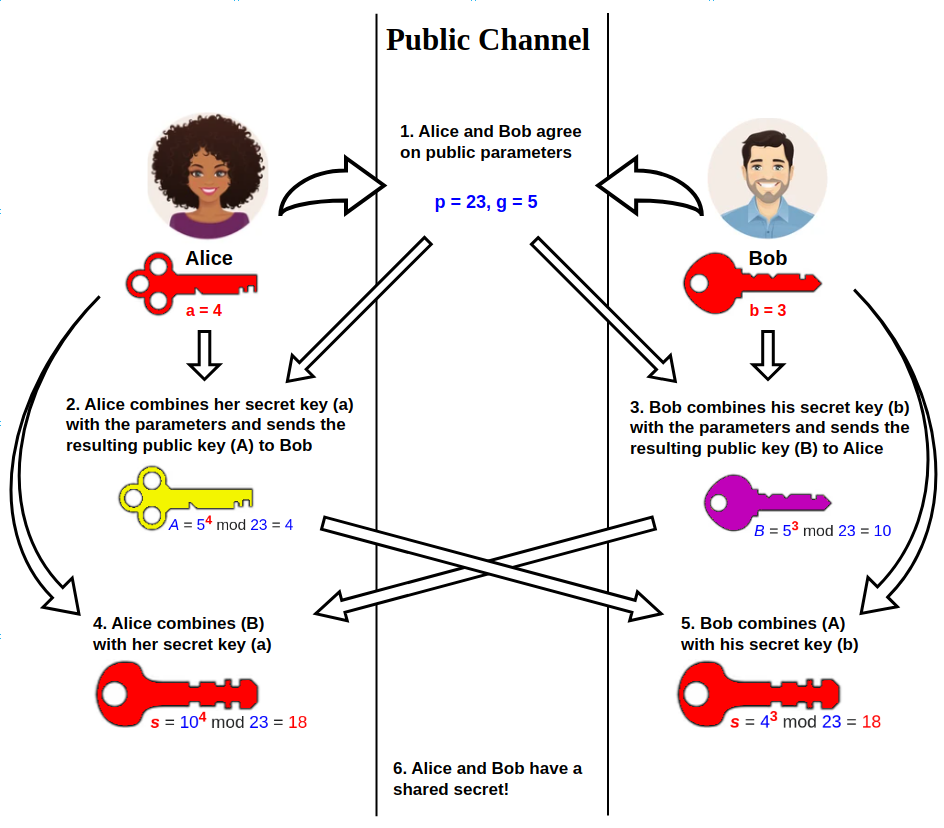
\includegraphics[height=\paperheight]{slide-images/dh-exchange}
    \caption{Epachamo via Wikimedia Commons}
    \label{fig:dh}
\end{figure}
\end{frame}

\begin{frame}\frametitle{Diffie-Hellman}
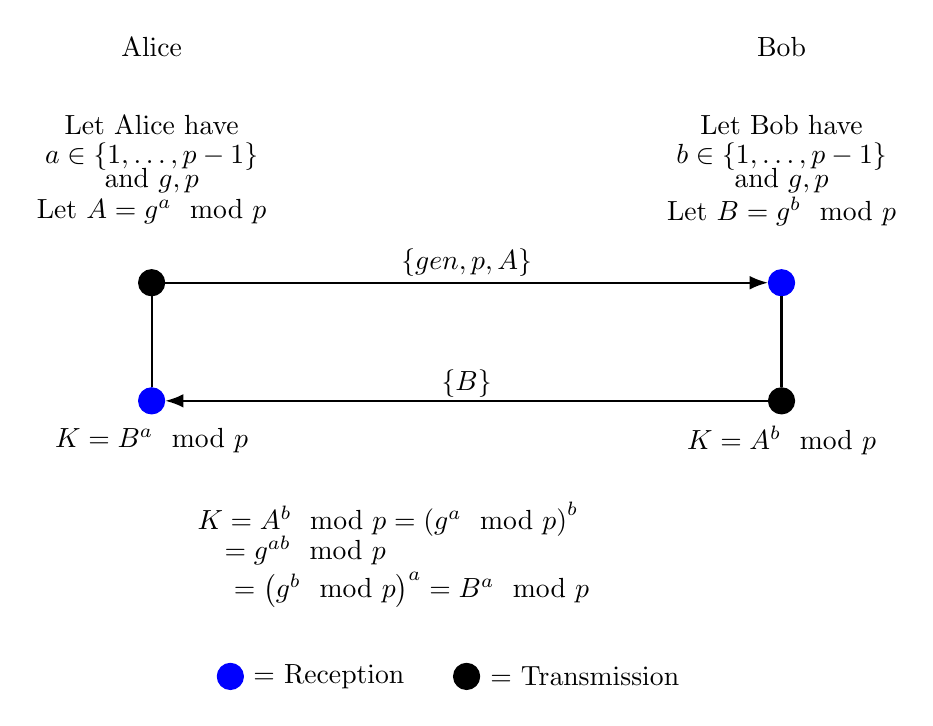
\begin{tikzpicture}
    \node at (0,8) {Alice};
    \node at (8,8) {Bob};
    \node[shape=circle,draw=blue, fill=blue] at (1,0) {};
    \node at (2.25,0) {= Reception};
    \node[shape=circle,draw=black, fill=black] at (4,0) {};
    \node at (5.5,0) {= Transmission};

    \pause
    \node at (0,7) {Let Alice have};
    \node at (0,6.6) {\(a \in \{1,\dots,p-1\}\)};
    \node at (0,6.3) {and \(g,p\)};
    \node at (0,5.9) {Let \(A = g^a \mod p\)};


    \node at (8,7) {Let Bob have};
    \node at (8,6.6) {\(b \in \{1,\dots,p-1\}\)};
    \node at (8,6.3) {and \(g,p\)};
    \node at (8,5.9) {Let \(B = g^b \mod p\)};
    
    \pause
    \node[shape=circle,draw=black, fill=black] (1) at (0,5) {};
    \node[shape=circle,draw=blue, fill=blue] (2) at (8,5) {};
    \path [saiarrow](1) edge (2);
    
    \node at (4,5.25) {\(\{gen,p,A\}\)};

    \node[shape=circle,draw=black, fill=black] (3) at (8,3.5) {};
    \node[shape=circle,draw=blue, fill=blue] (4) at (0,3.5) {};
    
    \path [-,thick](3) edge (2);
    \path [saiarrow](3) edge (4);
    \path [-,thick](1) edge (4);
    
    \node at (4,3.72) {\(\{B\}\)};

    \pause
    \node at (8,3) {\(K = A^b \mod p\)};
    \node at (0,3) {\(K = B^a \mod p\)};

    \node at (3,2) {\(K = A^b \mod p = \left(g^a \mod p\right)^b\)};
    \node at (1.95,1.6) {\(= g^{ab} \mod p \)};
    \node at (3.3,1.1) {\(= \left(g^b \mod p\right)^a = B^a \mod p\)};
\end{tikzpicture}
\end{frame}

\begin{frame}\frametitle{Diffie-Hellman Assumptions}
\pause
States that its computationally infeasible to compute \(g^{(ab)}\) even if \(g, g^a, g^b\) are known.

\pause
This is how it's possible to exchange keys using Diffie - Hellman securely.

\pause
There is a catch: 
\pause
whether it is actually computationally infeasible is not known, it is an open problem.
\end{frame}

\begin{frame}\frametitle{Some CPSA hints and notes}
\begin{itemize}
\item Need correct origination assumptions
\begin{itemize}
\item `a' and `b' (of sort \texttt{rndx}) need to be pen-non-orig
\item msg should be \texttt{uniq-orig} (if not it could lead to many shapes)
\end{itemize}
\item CPSA is used to find structural flaws, not algebraic flaws 
\pause
\item Now let's take a look at the model!
\end{itemize}
\end{frame}

\title{Reading Protocol Specifications}
\author{What do the keywords mean?}
\date{}
\begin{frame}
\maketitle
\end{frame}

\begin{frame}\frametitle{RFC 2119}
\begin{itemize}
\item Scott Bradner (March 1997) \href{https://datatracker.ietf.org/doc/html/rfc2119}{Key words for use in RFCs to Indicate Requirement Levels}
\pause
\item \textbf{MUST} indicates that a portion of the spec is absolutely required.
\pause
\item \textbf{MUST NOT} is an absolute prohibition of something.
\pause
\item \textbf{SHOULD} indicates that something is recommended.
\pause
\item \textbf{SHOULD NOT} indicates that something is not recommended.
\pause
\item \textbf{MAY} indicates that something is optional.
\end{itemize}
\end{frame}

\begin{frame}\frametitle{What really happens}
\begin{itemize}
\item \textbf{MUST} actually gets included
\pause
\item Nothing else is included \dots
\end{itemize}
\end{frame}

\begin{frame}\frametitle{Some tips for reading protocol specifications}

\begin{itemize}
\item FIND THE SECURITY GOALS
\item Find the messages
\begin{itemize}
\item ``The [party1] relays [data] to [party2]''
\item ``[party2] receives [data]'' (figure out who sent it)
\item ``With [data], [party2] does [action]'' (how did it get data?)
\end{itemize}
\item Find what every implementation must consider (\emph{MUST}\>), especially if you are comparing.
\item Find assumptions in the protocol (DY adversary)
\begin{itemize}
\item ``With private keys kept secret\dots''
\item ``We assume both clients are honest participants''
\item ``A high entropy source is available'' (\href{https://news.ycombinator.com/item?id=48060054}{UUID4})
\end{itemize}
\end{itemize}
\end{frame}

\begin{frame}\frametitle{Homework}
\pause
\begin{center}
{\Huge Capture the Flag Exercises}
\end{center}

Use CPSA to model protocols that are written in Python, identify the attack, and write the code needed to ``capture the flag'' (get the secret value out of the exchange).

\end{frame}


\begin{frame}\frametitle{Survey}
Fill in details about the survey here!
\end{frame}
\end{document}